\documentclass[dvips, lscape]{foils}
%\documentclass[dvips, french]{slides}
\textwidth 18.5cm
\textheight 25cm 
\topmargin -1cm 
\oddsidemargin  -1cm 
\evensidemargin  -1cm
% Maths
\usepackage{amsfonts, amsmath, amssymb, url}
\usepackage{/Latex/astats}

\newcommand{\coefbin}[2]{\left( 
    \begin{array}{c} #1 \\ #2 \end{array} 
  \right)}
\newcommand{\bbullet}{\bullet\bullet}
\newcommand{\bbbullet}{\bbullet\bullet}
\newcommand{\bbbbullet}{\bbbullet\bullet}
\newcommand{\Bcal}{\mathcal{B}}
\newcommand{\Ccal}{\mathcal{C}}
\newcommand{\Dcal}{\mathcal{D}}
\newcommand{\Ecal}{\mathcal{E}}
\newcommand{\Fcal}{\mathcal{F}}
\newcommand{\Gcal}{\mathcal{G}}
\newcommand{\Kcal}{\mathcal{K}}
\newcommand{\Mcal}{\mathcal{M}}
\newcommand{\Ncal}{\mathcal{N}}
\newcommand{\Pcal}{\mathcal{P}}
\newcommand{\Qcal}{\mathcal{Q}}
\newcommand{\Rcal}{\mathcal{R}}
\newcommand{\Scal}{\mathcal{S}}
\newcommand{\Hcal}{\mathcal{H}}
\newcommand{\Jcal}{\mathcal{J}}
\newcommand{\Lcal}{\mathcal{L}}
\newcommand{\Tcal}{\mathcal{T}}
\newcommand{\Ucal}{\mathcal{U}}
\newcommand{\Vcal}{\mathcal{V}}
\newcommand{\Xcal}{\mathcal{X}}
\newcommand{\Zcal}{\mathcal{Z}}
\newcommand{\dd}{\text{d}}
\newcommand{\etabar}{\overline{\eta}}
\newcommand{\pibar}{\overline{\pi}}
\newcommand{\alphabf}{\mbox{\mathversion{bold}{$\alpha$}}}
\newcommand{\betabf}{\mbox{\mathversion{bold}{$\beta$}}}
\newcommand{\gammabf}{\mbox{\mathversion{bold}{$\gamma$}}}
\newcommand{\mubf}{\mbox{\mathversion{bold}{$\mu$}}}
\newcommand{\nubf}{\mbox{\mathversion{bold}{$\nu$}}}
\newcommand{\phibf}{\mbox{\mathversion{bold}{$\phi$}}}
\newcommand{\pibf}{\mbox{\mathversion{bold}{$\pi$}}}
\newcommand{\Pibf}{\mbox{\mathversion{bold}{$\Pi$}}}
\newcommand{\psibf}{\mbox{\mathversion{bold}{$\psi$}}}
\newcommand{\Sigmabf}{\mbox{\mathversion{bold}{$\Sigma$}}}
\newcommand{\taubf}{\mbox{\mathversion{bold}{$\tau$}}}
\newcommand{\thetabf}{\mbox{\mathversion{bold}{$\theta$}}}
\newcommand{\xibf}{\mbox{\mathversion{bold}{$\xi$}}}
\newcommand{\Cbf}{{\bf C}}
\newcommand{\Ebf}{{\bf E}}
\newcommand{\Hbf}{{\bf H}}
\newcommand{\Ibf}{{\bf I}}
\newcommand{\Obf}{{\bf 0}}
\newcommand{\Pbf}{{\bf P}}
\newcommand{\Rbf}{{\bf R}}
\newcommand{\Sbf}{{\bf S}}
\newcommand{\Tbf}{{\bf T}}
\newcommand{\Ubf}{{\bf U}}
\newcommand{\mbf}{{\bf m}}
\newcommand{\ubf}{{\bf u}}
\newcommand{\vbf}{{\bf v}}
\newcommand{\Wbf}{{\bf W}}
\newcommand{\xbf}{{\bf x}}
\newcommand{\Xbf}{{\bf X}}
\newcommand{\Ybf}{{\bf Y}}
\newcommand{\ybf}{{\bf y}}
\newcommand{\zbf}{{\bf z}}
\newcommand{\Zbf}{{\bf Z}}
\newcommand{\Esp}{{\mathbb E}}
\newcommand{\Corr}{{\mathbb C}\mbox{orr}}
\newcommand{\Nbb}{\mathbb{N}}
\newcommand{\Nm}{N(\mbf)}
\newcommand{\mum}{\mu(\mbf)}
\newcommand{\obs}{\text{obs}}
\newcommand{\ERMG}{\text{EMRG}}
\newcommand{\Ibb}{{\mathbb I}}
\newcommand{\Omegas}{\underset{s}{\Omega}}
\newcommand{\Var}{{\mathbb V}}
\newcommand{\Pro}{\mathbb{P}}
\newcommand{\Rbb}{\mathbb{R}}
\newcommand{\RX}{R_{\Xbf}}
\newcommand{\Vsf}{\mathsf{V}}
\newcommand{\Starsf}{\mathsf{*}}
\newcommand{\QZ}{Q_{\Zbf}}
\newcommand{\QZi}{Q_{\Zbf_i}}
\newcommand{\Qt}{Q_{\thetabf}}
\newcommand{\logit}{\text{logit}}

% Couleur et graphiques
\usepackage{color}
\usepackage{graphics}
\usepackage{epsfig} 
\usepackage{pstcol}

% Texte
\usepackage{lscape}
\usepackage{../../../../Latex/fancyheadings, rotating, enumerate}
%\usepackage[french]{babel}
\usepackage[latin1]{inputenc}
%\definecolor{darkgreen}{cmyk}{0.5, 0, 0.5, 0.5}
%\definecolor{green}{cmyk}{0.5, 0, 0.5, 0.5}
\definecolor{orange}{cmyk}{0, 0.6, 0.8, 0}
\definecolor{jaune}{cmyk}{0, 0.5, 0.5, 0}
\newcommand{\textblue}[1]{\textcolor{blue}{#1}}
\newcommand{\textred}[1]{\textcolor{red}{#1}}
\newcommand{\textgreen}[1]{\textcolor{green}{ #1}}
\newcommand{\textlightgreen}[1]{\textcolor{green}{#1}}
%\newcommand{\textgreen}[1]{\textcolor{darkgreen}{#1}}
\newcommand{\textorange}[1]{\textcolor{orange}{#1}}
\newcommand{\textyellow}[1]{\textcolor{yellow}{#1}}
\newcommand{\emphase}[1]{\textblue{\sl #1}}
\newcommand{\refer}[1]{\textgreen{\sl \cite{#1}}}

% Listes
\newcommand{\itemv}{\item \vspace{-0.5cm}}

% Sections
%\newcommand{\chapter}[1]{\centerline{\LARGE \textblue{#1}}}
% \newcommand{\section}[1]{\centerline{\Large \textblue{#1}}}
% \newcommand{\subsection}[1]{\noindent{\Large \textblue{#1}}}
% \newcommand{\subsubsection}[1]{\noindent{\large \textblue{#1}}}
% \newcommand{\paragraph}[1]{\noindent {\textblue{#1}}}
% Sectionsred
\newcommand{\chapter}[1]{
  \addtocounter{chapter}{1}
  \setcounter{section}{0}
  \setcounter{subsection}{0}
  {\centerline{\LARGE \textblue{\arabic{chapter} - #1}}}
%  {\centerline{\LARGE \textblue{#1}}}
  }
\newcommand{\section}[1]{
  \addtocounter{section}{1}
  \setcounter{subsection}{0}
  {\noindent {\Large \textblue{\arabic{chapter}.\arabic{section} - #1}}}
%  {\noindent {\Large \textblue{#1}}}
  }
\newcommand{\subsection}[1]{
  \addtocounter{subsection}{1}
%   {\noindent{\large
%       \textblue{\arabic{chapter}.\arabic{section}.\arabic{subsection}
%         - #1}}}
  {\noindent{\large \textblue{#1}}}
  }
\newcommand{\paragraph}[1]{\noindent{\textblue{#1}}}

%%%%%%%%%%%%%%%%%%%%%%%%%%%%%%%%%%%%%%%%%%%%%%%%%%%%%%%%%%%%%%%%%%%%%%
%%%%%%%%%%%%%%%%%%%%%%%%%%%%%%%%%%%%%%%%%%%%%%%%%%%%%%%%%%%%%%%%%%%%%%
%%%%%%%%%%%%%%%%%%%%%%%%%%%%%%%%%%%%%%%%%%%%%%%%%%%%%%%%%%%%%%%%%%%%%%
%%%%%%%%%%%%%%%%%%%%%%%%%%%%%%%%%%%%%%%%%%%%%%%%%%%%%%%%%%%%%%%%%%%%%%
\begin{document}
%%%%%%%%%%%%%%%%%%%%%%%%%%%%%%%%%%%%%%%%%%%%%%%%%%%%%%%%%%%%%%%%%%%%%%
%%%%%%%%%%%%%%%%%%%%%%%%%%%%%%%%%%%%%%%%%%%%%%%%%%%%%%%%%%%%%%%%%%%%%%
%%%%%%%%%%%%%%%%%%%%%%%%%%%%%%%%%%%%%%%%%%%%%%%%%%%%%%%%%%%%%%%%%%%%%%
%%%%%%%%%%%%%%%%%%%%%%%%%%%%%%%%%%%%%%%%%%%%%%%%%%%%%%%%%%%%%%%%%%%%%%
\landscape
\newcounter{chapter}
\newcounter{section}
\newcounter{subsection}
\setcounter{chapter}{0}
\headrulewidth 0pt 
\pagestyle{fancy} 
\cfoot{}
\rfoot{
%   \begin{rotate}{90}{
%       \hspace{1cm} \tiny S. Robin: Statiscal Analysis of Interaction Graphs
%       }\end{rotate}
}
\rhead{\begin{rotate}{90}{
      \hspace{-.5cm} \tiny \thepage
      }\end{rotate}}

%%%%%%%%%%%%%%%%%%%%%%%%%%%%%%%%%%%%%%%%%%%%%%%%%%%%%%%%%%%%%%%%%%%%%%
%%%%%%%%%%%%%%%%%%%%%%%%%%%%%%%%%%%%%%%%%%%%%%%%%%%%%%%%%%%%%%%%%%%%%%
\begin{center}
  \textblue{\LARGE Some Statistical Aspects}

  \textblue{\LARGE of Interaction Network Analysis}

\end{center}

\hspace{-2cm}
\begin{tabular}{cc}
  \begin{tabular}{l}
    \textblue{\large S. Robin} \\
    ~\\
    {\tt robin@agroparistech.fr} \\
    ~\\~\\
    UMR 518 AgroParisTech / INRA \\
    Math�matique et Informatique \\
    Appliqu�es~: \\
    {\url{www.agroparistech.fr/mia/}}    
    ~\\~\\
    Statistics for Systems Biology \\
    (SSB) group: \\
    {\url{genome.jouy.inra.fr/ssb/}} \\
    ~\\
  \end{tabular}
  &
  \begin{tabular}{p{12cm}}
    \epsfig{file = ../Figures/Barabasi6.ps, clip=, bbllx=39, bblly=466,
      bburx=351, bbury=754, width=12cm, height=12cm}
  \end{tabular}
\end{tabular}



%%%%%%%%%%%%%%%%%%%%%%%%%%%%%%%%%%%%%%%%%%%%%%%%%%%%%%%%%%%%%%%%%%%%%
%%%%%%%%%%%%%%%%%%%%%%%%%%%%%%%%%%%%%%%%%%%%%%%%%%%%%%%%%%%%%%%%%%%%%
\newpage
\chapter{Introduction}
%%%%%%%%%%%%%%%%%%%%%%%%%%%%%%%%%%%%%%%%%%%%%%%%%%%%%%%%%%%%%%%%%%%%%
%%%%%%%%%%%%%%%%%%%%%%%%%%%%%%%%%%%%%%%%%%%%%%%%%%%%%%%%%%%%%%%%%%%%%

%%%%%%%%%%%%%%%%%%%%%%%%%%%%%%%%%%%%%%%%%%%%%%%%%%%%%%%%%%%%%%%%%%%%%
\section{Interaction Networks}
%%%%%%%%%%%%%%%%%%%%%%%%%%%%%%%%%%%%%%%%%%%%%%%%%%%%%%%%%%%%%%%%%%%%%
        
%%%%%%%%%%%%%%%%%%%%%%%%%%%%%%%%%%%%%%%%%%%%%%%%%%%%%%%%%%%%%%%%%%%%%
\subsection{Some examples}

\hspace{-2cm}
\begin{tabular}{cc}
  \begin{tabular}{p{12cm}}
    \paragraph{Social networks.} \\~\\
    Who loves who? Who's friend with who? \\~\\
    Which covariates contribute to explain the existence of a link? \\~\\~\\
    \paragraph{Industrial/commercial networks.} \\~\\
    Number of passenger exchanged between airports. \\~\\
  \end{tabular}
  &
  \begin{tabular}{p{12cm}}
    \paragraph{Biological networks.} \\~\\
    Which genes regulates which gene? Which proteins do interact (PPI)?\\~\\
    Does it help in understanding their biological function? \\~\\~\\
    \paragraph{Internet.}\\~\\
    How is it growing? \\~\\
    Do active website contain more relevant pieces of information? 
  \end{tabular}
\end{tabular}

%%%%%%%%%%%%%%%%%%%%%%%%%%%%%%%%%%%%%%%%%%%%%%%%%%%%%%%%%%%%%%%%%%%%%
\newpage
\subsection{Definitions}

\paragraph{An interaction network} is made of
\begin{itemize}
\itemv a set of $n$ \emphase{nodes} (vertices): $ i \in
  \Vcal = \{1, ... n\} $
\itemv a set of \emphase{edges}: $ \Ecal =
  \{X_{ij}\}_{i, j \in \Vcal} $
\end{itemize}

\bigskip\bigskip
\paragraph{Binary graph:}
If  $X_{ij} \in \{0, 1\} := \{\text{absent}, \text{present}\}$

\bigskip\bigskip
\hspace{-1.75cm}
\begin{tabular}{lll}
  \paragraph{Non-oriented graph:}
  If $X_{ij}$ is only defined & for $i < j$ & (no self-loop) \\
  & or $i \leq j$ & (self-loops).
\end{tabular}

\bigskip\bigskip
\paragraph{An oriented graph} can be represented as \emphase{multivariate
  valued non-oriented} graph, setting
$$
\tilde{X}_{ij} = (X_{ij}, X_{ji}) \qquad \text{for } i \leq j.
$$

\bigskip\bigskip
\paragraph{Notation for the whole graph:} $\Xcal = \{X_{ij}\}$.

%%%%%%%%%%%%%%%%%%%%%%%%%%%%%%%%%%%%%%%%%%%%%%%%%%%%%%%%%%%%%%%%%%%%%
\newpage
\subsection{Back to examples}

\noindent
\begin{tabular}{p{4.5cm}p{3.5cm}p{7cm}p{7.25cm}}
  Network & Nodes & Edges & Type \\
  \\
  \hline
  \\
  \paragraph{PPI} & Proteins & Physical interaction & binary,
  non-oriented (?) \\ 
  \\
  \paragraph{Social network} & People & Reciprocal~affinity \qquad (+
  covariates ?) & binary,  non-oriented \\ 
  \\
  \paragraph{Internet} & Websites & Links & binary, oriented \\
  \\
  \paragraph{Transportation} & Airports & Number of passengers &
  valued, oriented \\ 
  \\
  \paragraph{Ecology} & Tree species & Number of common parasites &
  valued, non-oriented \\ 
  \\
  \paragraph{Gene regulation} & Genes & Up/down regulation &
  binary/valued, oriented \\ 
\end{tabular}

%%%%%%%%%%%%%%%%%%%%%%%%%%%%%%%%%%%%%%%%%%%%%%%%%%%%%%%%%%%%%%%%%%%%%
\newpage
%\vspace{-2cm}
\begin{tabular}{ll}
  \hspace{-2cm}
  \begin{tabular}{p{12cm}}
    \subsection{Two representations}\\
    \subsection{= Two way of thinking?}\\
    \\
    \paragraph{Graph representation.}
    \begin{itemize}
    \itemv Easy to read
    \itemv Interpretation in terms of \emphase{relative
        positions} of the nodes ... that are arbitrary
    \end{itemize}
  \end{tabular}
  &
  \begin{tabular}{c}
  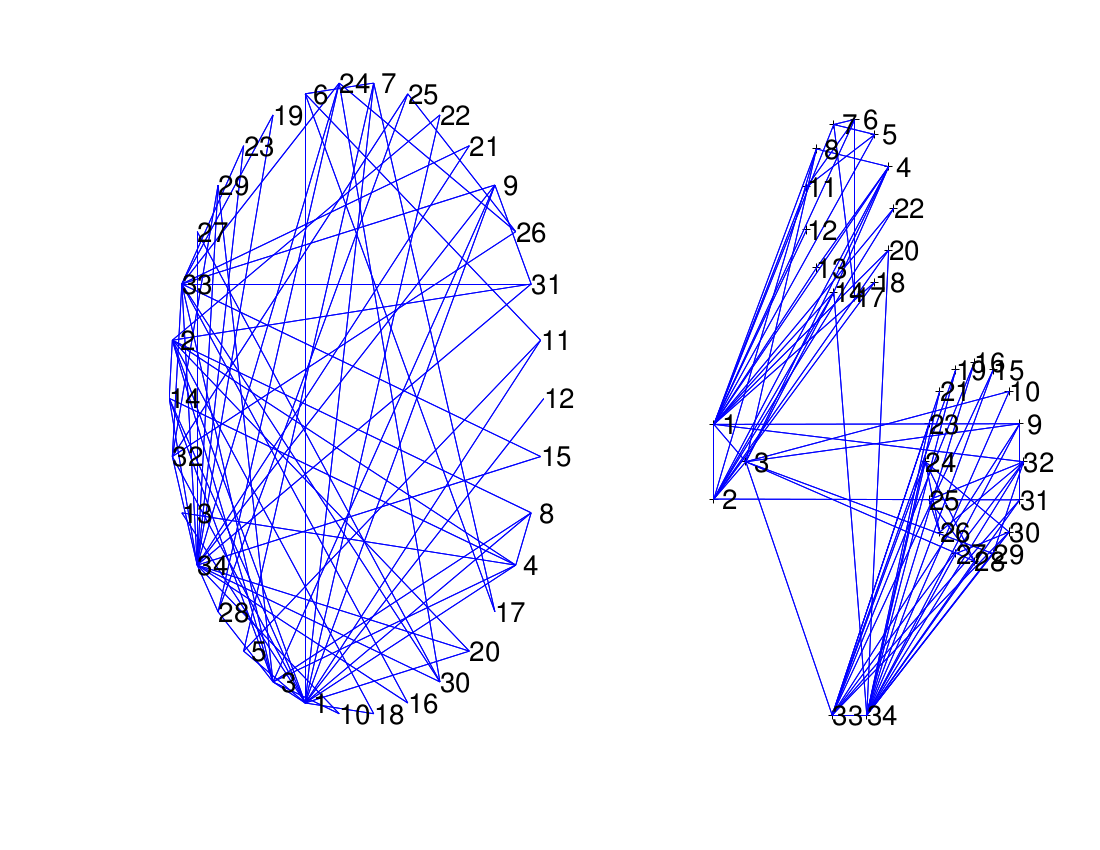
\epsfig{file = ../Figures/Karate-Graph.eps, clip=, width=7cm,
    height=10cm, angle=270, bbllx=50, bblly=100, bburx=530, bbury=400}
  \end{tabular}
  \\
  \hspace{-2cm}
  \begin{tabular}{p{12cm}}
    \paragraph{Adjacency matrix.}
    \begin{itemize}
    \itemv Difficult to read
    \itemv Closer to the \emphase{statistical data
        structure}
    \itemv Row and column ordering is still arbitrary.
    \end{itemize}
  \end{tabular}
  &
  \begin{tabular}{c}
    \qquad
    \epsfig{file = ../Figures/Karate-Dotplot.eps, clip=, width=7cm,
      height=8cm, angle=270, bbllx=50, bblly=100, bburx=530, bbury=400}
  \end{tabular}
\end{tabular}

%%%%%%%%%%%%%%%%%%%%%%%%%%%%%%%%%%%%%%%%%%%%%%%%%%%%%%%%%%%%%%%%%%%%%
\newpage
\section{Random Graph Model}
%%%%%%%%%%%%%%%%%%%%%%%%%%%%%%%%%%%%%%%%%%%%%%%%%%%%%%%%%%%%%%%%%%%%%

%%%%%%%%%%%%%%%%%%%%%%%%%%%%%%%%%%%%%%%%%%%%%%%%%%%%%%%%%%%%%%%%%%%%
\subsection{A huge probabilistic literature ...}

Since the first works of \emphase{Erd�s \& R�nyi}, the
probabilistic properties of random graphs have been intensively
studied.

Typical quantities of interest are
\begin{itemize}
\itemv the node degrees (scale-free distribution?), 
\itemv the network diameter (small-world effect?),
\itemv the number of triangles and/or the clustering
  coefficient,
\itemv the number of connected components and the size
  of the largest one,
\itemv the spread of an epidemic or an innovation.
\end{itemize}
Numerous asymptotic and exact results are available, for large
classes of random graphs. \\
See \refer{PaR07} for a general review on random graph models.
%PaR07-SAGE.pdf

%%%%%%%%%%%%%%%%%%%%%%%%%%%%%%%%%%%%%%%%%%%%%%%%%%%%%%%%%%%%%%%%%%%%
\newpage
\subsection{... But less in statistics}

Statistical tools to analyse network structured data seem to be much
more recent. \\ ~\\
\begin{tabular}{lc}
  Network data do not have the structure  &
  \emphase{individuals $\times$ variables} \\
  \\
  but rather &
  \emphase{individuals $\times$ individuals} \\
  \\
  or even &
  \emphase{individuals $\times$ individuals $\times$ variables}
\end{tabular}

\bigskip\bigskip
\paragraph{Outline:} Very \emphase{non-exhaustive} overview ony
\begin{itemize}
\itemv Some Random Graph Models 
\itemv Fitting a Model to an Observed Network
\itemv Describing (Local) Structure
\itemv Network inference
\end{itemize}

%%%%%%%%%%%%%%%%%%%%%%%%%%%%%%%%%%%%%%%%%%%%%%%%%%%%%%%%%%%%%%%%%%%%%
%%%%%%%%%%%%%%%%%%%%%%%%%%%%%%%%%%%%%%%%%%%%%%%%%%%%%%%%%%%%%%%%%%%%%
\newpage
\chapter{Some Random Graph Models}
%%%%%%%%%%%%%%%%%%%%%%%%%%%%%%%%%%%%%%%%%%%%%%%%%%%%%%%%%%%%%%%%%%%%%
%%%%%%%%%%%%%%%%%%%%%%%%%%%%%%%%%%%%%%%%%%%%%%%%%%%%%%%%%%%%%%%%%%%%%

%%%%%%%%%%%%%%%%%%%%%%%%%%%%%%%%%%%%%%%%%%%%%%%%%%%%%%%%%%%%%%%%%%%%%
\section{Erd�s-R�nyi}
%%%%%%%%%%%%%%%%%%%%%%%%%%%%%%%%%%%%%%%%%%%%%%%%%%%%%%%%%%%%%%%%%%%%%
        
\paragraph{Model.} 
$$
\{X_{ij}\}_{1\leq i<j\leq n} \mbox{ i.i.d. } \sim \Bcal(\pi). 
$$

\bigskip\bigskip
\paragraph{Degree distribution.} Number of edges connected to node $i$:
$$
K_i := X_{i+} \sim \Bcal(n-1, \pi) \approx \Pcal[(n-1)\pi]
$$
where $X_{i+} := \sum_{j \neq i} X_{ij}$.

\bigskip\bigskip
\paragraph{Clustering coefficient.} Probability for two of my friends
to be friends:
\begin{eqnarray*}
c & = & \Pr\{\nabla | \mathsf{V}\} \\
& = & \Pr\{X_{ij} = 1 | X_{ik} = X_{jk} = 1\} \\
& = & \pi.
\end{eqnarray*}

%%%%%%%%%%%%%%%%%%%%%%%%%%%%%%%%%%%%%%%%%%%%%%%%%%%%%%%%%%%%%%%%%%%%%
\newpage
\paragraph{Likelihood.} $X_{++} = \sum_i X_{i+} = 2 \times $ number of edges:
\begin{eqnarray*}
  \Pr\{\Xcal\} & = & \pi^{X_{++}/2} (1-\pi)^{[n(n-1) - X_{++}]/2} \\
  \Lcal(\Xcal; \pi) & = & \frac{X_{++}}2 \log\pi + \frac{n(n-1) -
  X_{++}}2 \log(1-\pi) 
\end{eqnarray*}

\paragraph{Maximum likelihood estimate (MLE) of $\pi$.}
$$
\widehat{\pi} = \frac{X_{++}}{n(n-1)}.
$$


%%%%%%%%%%%%%%%%%%%%%%%%%%%%%%%%%%%%%%%%%%%%%%%%%%%%%%%%%%%%%%%%%%%%%
\newpage
\section{Degree distribution fitting}
%%%%%%%%%%%%%%%%%%%%%%%%%%%%%%%%%%%%%%%%%%%%%%%%%%%%%%%%%%%%%%%%%%%%%
        
%%%%%%%%%%%%%%%%%%%%%%%%%%%%%%%%%%%%%%%%%%%%%%%%%%%%%%%%%%%%%%%%%%%%%
\subsection{Fixed degree (FD)}

\paragraph{Model.} For a \emphase{given graph} $\Xcal_{\text{obs}}$ with
degree sequence $\Kcal = \{k_i\}_{i=1..n}$
$$
\Xcal \sim \Ucal_{\Gcal}, \qquad \text{where } \Gcal = \text{set of
  all graphs with degree sequence } \Kcal.
$$

\bigskip
\paragraph{Parameter.} Degree sequence $\Kcal$.

\bigskip\bigskip
\paragraph{Properties.}
\begin{itemize}
\itemv The degree of node $i$ is \emphase{not random}:
  $ K_i = k_i.  $
\itemv This model is \emphase{not stationary}:
  $
  \Pr\{X_{ij} = 1\} \neq \Pr\{X_{i'j'} = 1\}.
  $
% \itemv If self-loops are allowed
%   $\displaystyle{
%     \# \Gcal \approx \binom{x_{++}}{\underset{x_{++} \text{
%           times}}{\underbrace{\begin{array}{ccc}2 & \dots & 2
%           \end{array}}}}
%     = \frac{x_{++}!}{2^{x_{++}/2} }
%     }$
\end{itemize}

%%%%%%%%%%%%%%%%%%%%%%%%%%%%%%%%%%%%%%%%%%%%%%%%%%%%%%%%%%%%%%%%%%%%%
\newpage
\paragraph{2 sampling schemes.} 

\hspace{-2cm}
\begin{tabular}{cc}
  \begin{tabular}{p{12cm}}
    1 -- Each node $i$ is provided with $k_i$
    \emphase{semi-edges}: \\
%    $$
    \epsfig{file = ../Figures/FigFDD-SemiEdge.eps, width=10cm, clip=} \\
%    $$
    $\Xcal = $ \emphase{uniform sample} (without replacement) 
    of $k_{+}/2$ pairs among the $k_{+}$ semi-edges. \\
    \\
    (Problem if self-loops are forbidden.)
  \end{tabular}
  &
  \begin{tabular}{p{12cm}}
    2 -- Pick at random a pair of edges $x_{i_1 j_2}$ and
    $x_{i_2 j_2}$ and \emphase{rewire them}
    $$
    (x_{i_1 j_1}, x_{i_2 j_2}) \longrightarrow (x_{i_1 j_2}, x_{i_2 j_1})
    $$
    $$
    \epsfig{file = ../Figures/FigFDD-Rewire-1.eps, width=5cm,
      height=5cm, clip=}  
    \hspace{2cm}
    \epsfig{file = ../Figures/FigFDD-Rewire-2.eps, width=5cm,
      height=5cm, clip=} 
    $$
    so that the degrees $k_{i_1}$, $k_{i_2}$, $k_{j_1}$ and $k_{j_2}$
    are unchanged. \\ 
    ~\\
    Iterate rewiring a \emphase{'large number of times'} to get an
    independent copy.
    \\ ~\\
  \end{tabular}
\end{tabular}

%%%%%%%%%%%%%%%%%%%%%%%%%%%%%%%%%%%%%%%%%%%%%%%%%%%%%%%%%%%%%%%%%%%%%
\newpage
\subsection{Expected degree (ED) model} 

\paragraph{Model.} For an \emphase{given graph} $\Xcal_{\text{obs}}$
with degree sequence $\Kcal = \{k_i\}_{i=1..n}$,
$$
\{X_{ij}\} \text{ independent}, \quad X_{ij} \sim \Bcal(\pi_{ij}), \qquad
\pi_{ij} = \lambda k_i k_j
$$
with $\lambda^{-1} = (n-1) \overline{k}$ to ensure $\Esp K_i = k_i$.

%%%%%%%%%%%%%%%%%%%%%%%%%%%%%%%%%%%%%%%%%%%%%%%%%%%%%%%%%%%%%%%%%%%%%
\bigskip\bigskip\bigskip
\subsection{Expected degree distribution (EDD) model}

\paragraph{Model.} Expected degrees $\{D_i\}$ are i.i.d. with \emphase{given
  degree distribution} (e.g. the empirical degree distribution of
$\Xcal_{\text{obs}}$),
$$
\{X_{ij}\} \text{ independent } | \{D_i\}, \quad X_{ij}|(D_i, D_j)
\sim \Bcal(\pi_{ij}), \qquad \pi_{ij} = \lambda D_i D_j
$$
with $\lambda^{-1} = (n-1) \Esp D_i$ to ensure $\Esp(K_i | D_i) =
D_i$. \\
\\
$\Rightarrow$ The expected distribution $p(k)$ is preserved, but
\emphase{not the degree of each node}.

%%%%%%%%%%%%%%%%%%%%%%%%%%%%%%%%%%%%%%%%%%%%%%%%%%%%%%%%%%%%%%%%%%%%%
\newpage
\hspace{-1.75cm}
\begin{tabular}{rl}
  \paragraph{Parameter.} \qquad 
  ED model: & Degree sequence $\Kcal$ \\
  \\
  EDD model: & Degree distribution $p(k)$
\end{tabular}

\bigskip\bigskip
\paragraph{Properties.}
\begin{itemize}
\itemv \emphase{Degrees are random}: 
  $$
  \Esp_{\text{ED}}(K_i) = k_i,
  $$
  $$
  \Esp_{\text{EDD}}(K_i|D_i) = D_i, \qquad
  \Esp_{\text{EDD}}(K_i) = \Esp_p(D_i). 
  $$
\itemv \emphase{EDD is stationary}, i.e. the joint distribution of the
  edges between a subset $\Scal$ is the same for all subset of same
  size:
  $$
  \forall \Scal, \Scal' \subset \Vcal, 
  \qquad |\Scal| = |\Scal'|, 
  \qquad \{X_{ij}\}_{i, j \in \Scal} \overset{\Dcal}{=} \{X_{ij}\}_{i, j
        \in \Scal'} 
  $$ 
  (\emphase{while ED is not}).
\end{itemize}


%%%%%%%%%%%%%%%%%%%%%%%%%%%%%%%%%%%%%%%%%%%%%%%%%%%%%%%%%%%%%%%%%%%%%
\newpage
\section{Preferential attachment}
% BaA99-Science.pdf
%%%%%%%%%%%%%%%%%%%%%%%%%%%%%%%%%%%%%%%%%%%%%%%%%%%%%%%%%%%%%%%%%%%%%

\paragraph{(Basic) model.} \refer{BaA99}
\begin{itemize}
\itemv Starting from $m_0 \geq m$ initial nodes.
\itemv Nodes \emphase{enter the network one by one}.
  Let $K_i^j$ denote the degree of node $i$ at 'time' $j$ (i.e.  when
  the network has size $j$):
  $$
  K_i^j = \sum_{\ell=1}^j X_{i\ell},
  $$
\itemv Node $j+1$ is connected to \emphase{$m$ older
    nodes}, with probability proportional to their current degree
  (\emphase{rich-get-richer}):
  $$
  \Pr\{X_{i, j+1} = 1\} \propto K_i^j, 
  $$
  i.e. the connexions of node $j+1$ are sampled among the $j$
  preceeding nodes with \emphase{unequal probabilities} ($\propto
  K_i^j$) and \emphase{without replacement}.
\end{itemize}

%%%%%%%%%%%%%%%%%%%%%%%%%%%%%%%%%%%%%%%%%%%%%%%%%%%%%%%%%%%%%%%%%%%%%
\newpage
\paragraph{Properties.}
\begin{itemize}
  \itemv Degrees have a \emphase{power-law} (\emphase{scale-free})
  distribution:
  $$
  p(k) \propto m^2/k^3
  $$
  (which is not defined for $k=0$)
\itemv Sub-sample of 'scale-free' networks are not scale-free (\refer{SWM05}).
\end{itemize}

\hspace{-2cm}
\begin{tabular}{cc}
  \begin{tabular}{p{14cm}}
    \paragraph{Parameter inference.} The parameter of the basic model is
    $m$ (and $m_0$). \\
    \\
    However, inference is generally focused on the \emphase{exponent
      $\alpha$} such that $p(k) \propto k^{-\alpha}$. \\
    \\
    The assessment of the scale-free distribution and the estimation of
    $\alpha$ are often based on the \emphase{log-log plot} of the
    degree distribution (\refer{BaA99}). 
  \end{tabular}
  &
  \begin{tabular}{p{10cm}}
    \paragraph{World-wide web} degree dist. \\
    %\epsfig{file = ../figures/log_log.eps, height=8cm, width = 8cm}
    \epsfig{file=../Figures/BaA99-Science-2.ps, clip=, width=8cm,
    height=8cm, bbllx=170, bblly=120, bburx=270, bbury=250}
  \end{tabular}
\end{tabular}


%%%%%%%%%%%%%%%%%%%%%%%%%%%%%%%%%%%%%%%%%%%%%%%%%%%%%%%%%%%%%%%%%%%%%
\newpage
\section{Exponential Random Graph Models (ERGM)}
%%%%%%%%%%%%%%%%%%%%%%%%%%%%%%%%%%%%%%%%%%%%%%%%%%%%%%%%%%%%%%%%%%%%%

\paragraph{Model.} Denoting $\Xbf = \{x_{ij}\}_{i, j}$:
$$
\Pr\{\Xbf = \xbf\} \propto \exp g(\xbf; \gammabf), 
\qquad \text{where } g(\xbf; \gammabf) = \sum \gamma_a s_a(\xbf)
$$
where the $s_a$ are \emphase{(sufficient) statistics}, associated
with parameters $\gammabf = (\gamma_a)$ (\refer{PaR07}, also called
\emphase{'P$^*$' models}).
%PaR07-SAGE.pdf

\bigskip
\paragraph{Typical statistics:} Number of edges, $\mathsf{V}$, triangles, etc.

\bigskip\bigskip
\paragraph{Simulation.} Simulation of ERMG is not straightforward,
particularly because of the normalising constant. A
\emphase{Metropolis-Hastings algorithm} can be used where, at each
  step:
\begin{itemize}
\itemv $\xbf$ is transformed into $\xbf'$ by switching a randomly chosen
  edge: $x'_{ij} = 1 - x_{ij}$;
\itemv  $\xbf$ is replaced by $\xbf'$ with probability $\min \left(1,
  \exp\left\{ \sum_a \gamma_a [s_a(\xbf') - s_a(\xbf)] \right\} \right)$.
\end{itemize}

%%%%%%%%%%%%%%%%%%%%%%%%%%%%%%%%%%%%%%%%%%%%%%%%%%%%%%%%%%%%%%%%%%%%%
\newpage
\section{Latent space}
%%%%%%%%%%%%%%%%%%%%%%%%%%%%%%%%%%%%%%%%%%%%%%%%%%%%%%%%%%%%%%%%%%%%%

\paragraph{General definition for binary graphs.} (\refer{BJR07})
% BJR07-RandStructAlgo.pdf        
\begin{itemize}
\item \vspace{-0.5cm} $n$ nodes $(i = 1 \dots n$)
\item \vspace{-0.5cm} $n(n-1)/2$ possible edges: $X_{ij} = \Ibb\{ i \sim j\}$
\item \vspace{-0.5cm} Each $i$ is characterised by a \emphase{latent
    variable} $Z_i$ sampled in some space $\Zcal$ with distribution
  $\alpha$:
  $$
  \{Z_i\}_i \mbox{ i.i.d.}, \qquad Z_i \sim \alpha
  $$
\item \vspace{-0.5cm} Edge $(i, j)$ is present with probability
  $\pi(Z_i, Z_j)$, where $\pi$ is a \emphase{kernel function}:
  $$
  \{X_{ij}\}_{i, j} \mbox{ independent given } \{Z_i\}_i, \qquad X_{ij}
  \sim \Bcal[\pi(Z_i, Z_j)].
  $$
\end{itemize}
\paragraph{Latent space:} 
$\displaystyle{
\Zcal = \Rbb^k, \qquad \logit[\pi(z, z')] :=
\log\left(\frac{\pi}{1-\pi}\right) = a - |z-z'|
}. 
$

\paragraph{Mixture model:} 
$\displaystyle{
\Zcal = \{1, \dots, Q\}, \qquad \pi(z, z') = \pi_{q\ell} \mbox{ for } z
= q, z' = \ell.
}$


%%%%%%%%%%%%%%%%%%%%%%%%%%%%%%%%%%%%%%%%%%%%%%%%%%%%%%%%%%%%%%%%%%%%%
%%%%%%%%%%%%%%%%%%%%%%%%%%%%%%%%%%%%%%%%%%%%%%%%%%%%%%%%%%%%%%%%%%%%%
\newpage
\chapter{Fitting a Model to an Observed Network}
%%%%%%%%%%%%%%%%%%%%%%%%%%%%%%%%%%%%%%%%%%%%%%%%%%%%%%%%%%%%%%%%%%%%%
%%%%%%%%%%%%%%%%%%%%%%%%%%%%%%%%%%%%%%%%%%%%%%%%%%%%%%%%%%%%%%%%%%%%%

%%%%%%%%%%%%%%%%%%%%%%%%%%%%%%%%%%%%%%%%%%%%%%%%%%%%%%%%%%%%%%%%%%%%%
\section{Exponential Random Graph Model}
%%%%%%%%%%%%%%%%%%%%%%%%%%%%%%%%%%%%%%%%%%%%%%%%%%%%%%%%%%%%%%%%%%%%%

%%%%%%%%%%%%%%%%%%%%%%%%%%%%%%%%%%%%%%%%%%%%%%%%%%%%%%%%%%%%%%%%%%%%%
\subsection{Pseudo-Likelihood}

\paragraph{MLE.} The maximisation of the log-likelihood
$$
\Lcal(\xbf; \gammabf) = g(\xbf; \gammabf) - \log \sum_{\xbf'} \exp
g(\xbf'; \gammabf)
$$
is intractable, mainly because of the normalizing constant.

\bigskip\bigskip
\paragraph{Pseudo-MLE.} The idea is to approximate $\Lcal(\xbf;
\gammabf)$ (\refer{WaP96}):
$$
\Lcal(\xbf; \gammabf) \approx \log\left(\prod_{ij} \Pr\{X_{ij}=x_{ij}
  | \Cbf_{ij}\} \right)
$$
where $\Cbf_{ij}$ stands for the complementary of $X_{ij}$ in the
graph $\Xbf$: $\Cbf_{ij} = \Xbf \setminus X_{ij}$.

%%%%%%%%%%%%%%%%%%%%%%%%%%%%%%%%%%%%%%%%%%%%%%%%%%%%%%%%%%%%%%%%%%%%%
\newpage
\bigskip\bigskip
\paragraph{Conditional distribution of one edge.} Denoting
\begin{itemize}
\itemv $\Xbf_{ij}^+$ the graph $\Xbf$ where $X_{ij}$ is set to 1,
\itemv $\Xbf_{ij}^-$ the graph $\Xbf$ where $X_{ij}$ is set to 0,
\end{itemize}
$\begin{array}{lcl}
  \text{we have} \qquad 
\logit~\Pr\{X_{ij} = 1 | \Cbf_{ij}\} & = &   \log
  \left(\Pr\{\Xbf_{ij}^+\} / \Pr\{\Xbf_{ij}^-\} \right) \\
  \\
  & = & g(\Xbf_{ij}^-; \gammabf) - g(\Xbf_{ij}^+; \gammabf) \\
  \\
  & = & \sum_a \gamma_a [s_a(\Xbf_{ij}^+) - s_a(\Xbf_{ij}^-)].
\end{array}$

\bigskip\bigskip
\paragraph{Logistic regression.} ERGM pseudo-MLE of $\gammabf$ is
hence equivalent to MLE estimate of a logistic regression with covariates
$$
\xi_{ij, a} = s_a(\Xbf_{ij}^+) - s_a(\Xbf_{ij}^-).
$$
\refer{LuS07} mention that the pseudo-likelihood works well in
practice but seems to underestimate the variance of the estimates.


%%%%%%%%%%%%%%%%%%%%%%%%%%%%%%%%%%%%%%%%%%%%%%%%%%%%%%%%%%%%%%%%%%%%%
\newpage
\subsection{(Monte Carlo) Maximum Likelihood}

\paragraph{MLE can be derived,} but some quantity need to be estimated via a MC
step:
$$
$$

% 1 - Snijders, Tom A.B. 2002. Markov Chain Monte Carlo Estimation of
% Exponential Random Graph Models. Journal of Social Structure, 3.2. Web
% journal available from 
% http://www2.heinz.cmu.edu/project/INSNA/joss/index1.html.

% 2 - Snijders, Tom A.B., and Mark Huisman. 2003. Manual for SIENA version
% 1.98. Groningen: ICS.

\bigskip\bigskip
\subsection{Bayesian / MCMC}

\bigskip
\paragraph{Gibbs sampling.}
Random $\Xbf$ can be generated by iteratively sampling each edge
conditionally to the others, according to
$$
P(X_{ij} | \Cbf_{ij})
$$
that has a simple form.

\bigskip\bigskip
\paragraph{Finding good proposals} for the parameters is still an
'art' (\refer{SPR06}).

%\refer{SaF07}
% SaF07-Bioinfo.pdf

%\refer{RSW07}
% RSW07-SocNet.pdf


% http://www.sna.unimelb.edu.au/publications/publications.html
%
% 1 - Wasserman, S., & Pattison, P. (1996). Logit models and logistic
% regressions for social networks, I. An introduction to Markov graphs
% and p *. Psychometrika 61 : 401-425.
%
% 2 - Pattison, P, & Wasserman, S. (1999) Logit models and logistic
% regressions for social networks, II. Multivariate relationships.
% British Journal of Mathematical and Statistical Psychology 52 :
% 169-193.
%
% 3 - Robins, G., Pattison, P., & Wasserman, S. (1999) Logit models and
% logistic regressions for social networks, III. Valued relations.
% Psychometrika 64 : 371-394.

%%%%%%%%%%%%%%%%%%%%%%%%%%%%%%%%%%%%%%%%%%%%%%%%%%%%%%%%%%%%%%%%%%%%%
\newpage
\subsection{ABC Inference for Evolutionary Network}

\bigskip
\paragraph{\refer{RJH07}} propose a model to describe the evolution of a
PPI network.

\bigskip\bigskip
\hspace{-2cm}
\begin{tabular}{cc}
  \begin{tabular}{p{14cm}}
    \paragraph{Model.} At each time $t$, a new node joins the network
    either according to a
    \begin{itemize}
      \itemv \emphase{duplication divergence} with parent-child
      attachment (DDa: prob. $\alpha$) \itemv or to
      \emphase{preferential attachment} (PA: prob. $1-\alpha$))
    \end{itemize}
  \end{tabular}
  &
  \begin{tabular}{p{10cm}}
    \centerline{
                                % RJH07-PLoSCompBiol.pdf
      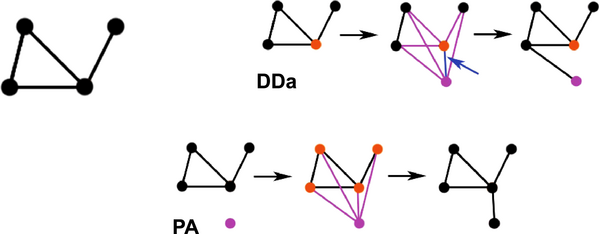
\epsfig{file=../Figures/RJH07-PLoSCompBiol-Fig7.ps, width=9cm,
        height=4cm, bbllx=255, bblly=150, bburx=580, bbury=240, clip=}
      }
  \end{tabular}
\end{tabular}

\bigskip
\paragraph{Likelihood.} Since the history of the network is not
observed, the likelihood is a \emphase{sum over all possible paths}
that could give raise to the observed network.

Direct ML can not be achieved.

%%%%%%%%%%%%%%%%%%%%%%%%%%%%%%%%%%%%%%%%%%%%%%%%%%%%%%%%%%%%%%%%%%%%%
\newpage
\paragraph{ABC inference.} A \emphase{likelihood-free} approach for an
observed network $\xbf$, consists in
\begin{itemize}
\itemv Defining a set $S$ of statistics, e.g.: number of edges,
  $\mathsf{V}$, triangles, etc.;
\itemv Sampling a value for parameter $\theta$ from a given prior;
\itemv Simulating a random network $\Xbf$ with same size as $\xbf$ xith
  parameter $\theta$;
\itemv Accepting $\theta$ if $\Xbf$ is similar to $\xbf$ in terms of $S$.
\end{itemize}

This sampling scheme provides an estimate of the
conditional distribution
$$
P(\theta | d[S(\xbf), S(\theta)] \leq \varepsilon)
\overset{?}{\approx}
P(\theta | \xbf).
$$

\paragraph{Remarks.}
\begin{enumerate}
\itemv The proposed algorithm looks like a Metropolis-Hastings for a
  \emphase{ERGM with same statistics $S$ and fixed parameter
    $\gammabf$} (summarised in the choice of the distance).
\itemv The calculation of the statistics $S$ for each simulated graph
  remains an \emphase{algorithmic issue}.
\end{enumerate}

% RJH07-PLoSCompBiol.pdf       

% To study the relative importance of aspects of duplication
% divergence in network evolution between different domains,
% we simulated the evolutionary history of PINs with a mixture
% of duplication divergence with parent�child attachment
% (DDa) and preferential attachment (PA); see Box 1. At each
% step, the network either grows according to DDa with
% probability 1  a or PA with probability a. More precisely,
% let Gt be a network with t nodes (proteins), v a new node, u a
% randomly chosen parent node in Gt, dDiv the divergence
% probability, dAtt the parent�child attachment probability, and
% let h � (dDiv, dAtt, a). Then the probability of Gt�1 conditional
% on Gt and u is
% P�Gt�1jGt; u; h� � aPA�u; v� � �1  a�DDa�u; v; dDiv; dAtt�: �1�
% The terms PA(u, v) and DDa(u, v, dDiv, dAtt) correspond to
% the probabilities of moving to the new configuration under PA and DDa, respectively. They are explained in Box 1 and
% defined fully in Protocol S1. By repeated application of the
% mechanism in Equation 1, we grew PINs to the approximate
% number of open reading frames in the respective genomes (H.
% pylori: 1,500, and P. falciparum: 5,300).

%%%%%%%%%%%%%%%%%%%%%%%%%%%%%%%%%%%%%%%%%%%%%%%%%%%%%%%%%%%%%%%%%%%%%
\newpage
\section{Latent space model}
%%%%%%%%%%%%%%%%%%%%%%%%%%%%%%%%%%%%%%%%%%%%%%%%%%%%%%%%%%%%%%%%%%%%%

\paragraph{Model.} 
\refer{HRH02}
% HRH02-JASA.pdf, 
\begin{itemize}
\itemv Each node has a \emphase{(unknown) position $\Zbf_i$ in a latent
  space} (euclidian, e.g. $\Rbb^d$):
  $$
  \{\Zbf_i\} \text{ i.i.d.} \sim F \qquad(\text{e.g. } F = \Ncal(\Obf,
  \Sigmabf)). 
  $$
\itemv Edges $\{X_{ij}\}_{i, j}$ are independent, conditionally on
  $\{Z_i\}$: 
  $$
  X_{ij} \sim \Bcal(\pi_{ij}), 
  \qquad \logit(\pi_{ij}) = a + \|\Zbf_i -
  \Zbf_j\|. 
  $$
\end{itemize}

\paragraph{Covariates can be added:}
$
\qquad
\displaystyle{\log\left(\frac{\pi_{ij}}{1-\pi_{ij}}\right) = a +
  \xibf_{ij} \thetabf + \|\Zbf_i - \Zbf_j\|}.
$

%%%%%%%%%%%%%%%%%%%%%%%%%%%%%%%%%%%%%%%%%%%%%%%%%%%%%%%%%%%%%%%%%%%%%
\newpage
\paragraph{Identifiability.} The estimation of $\Zcal = \{\Zbf_{ij}\}$
is a \emphase{Multidimensional Scaling} problem, that is not
identifiable. \refer{HRH02} use a Procustean trick to select each
configuration.

\bigskip\bigskip
\paragraph{Inference.} The authors adopt a Bayesian strategy using a
Metropolis-Hastings algorithm including conditional sampling steps
\begin{enumerate}
\itemv $\widehat{\Zcal} | (\widehat{a}, \widehat{\thetabf})$,
\itemv $(\widehat{a}, \widehat{\thetabf}) | \widehat{\Zcal}$.
\end{enumerate}

\bigskip\bigskip
\paragraph{Remarks.} 
\begin{itemize}
\itemv A frequentist approach could work, using an E-M strategy but the
  sampling of $\widehat{\Zcal} | (\widehat{a}, \widehat{\thetabf})$
  would probably require a Monte-Carlo step.
\itemv New version of the model and of the algorithm: \refer{HRT07}
\end{itemize}

%%%%%%%%%%%%%%%%%%%%%%%%%%%%%%%%%%%%%%%%%%%%%%%%%%%%%%%%%%%%%%%%%%%%%
\newpage
\section{Mixture model}
%%%%%%%%%%%%%%%%%%%%%%%%%%%%%%%%%%%%%%%%%%%%%%%%%%%%%%%%%%%%%%%%%%%%%

\bigskip
\paragraph{Model.} Each node has an \emphase{unobserved label} $Z_i$:
$$
\{Z_i\}_i \mbox{ i.i.d.}, \qquad Z_i \sim \Mcal(1; \alphabf)
$$
where $\alphabf = (\alpha_1, \dots \alpha_Q)$; The values of the edges
$\{X_{ij}\}_{i, j}$ are conditionally independent given the $Z_i$'s:
$$
(X_{ij} \;|\; Z_i = q, Z_j = \ell) \sim f_{q\ell}(\cdot).
$$
where $f_{q\ell}(\cdot)$ is some parametric distribution
$f_{q\ell}(x) = f(x; \theta_{q\ell})$. \\
Hidden labels account for \emphase{heterogeneous connexion profiles}
of the nodes.

\bigskip\bigskip
\paragraph{Inference.}
\begin{itemize}
\itemv {Bayesian / MCMC inference:} \refer{NoS01}
\itemv {Approximate (variational) ML:} \refer{DPR08}
\end{itemize}


%%%%%%%%%%%%%%%%%%%%%%%%%%%%%%%%%%%%%%%%%%%%%%%%%%%%%%%%%%%%%%%%%%%%%
\newpage
\section{Accounting for Covariates}
%%%%%%%%%%%%%%%%%%%%%%%%%%%%%%%%%%%%%%%%%%%%%%%%%%%%%%%%%%%%%%%%%%%%%

%%%%%%%%%%%%%%%%%%%%%%%%%%%%%%%%%%%%%%%%%%%%%%%%%%%%%%%%%%%%%%%%%%%%%
\subsection{Problem}

\noindent Describe the influence of covariates on the
presence/absence or the values of the edges.

\bigskip\bigskip
\paragraph{Example for social network.} For a network describing
social relations between students $i = 1, ..., n$, one observe for
student $i$ the vector of covariates
$$
\xibf_i = (\xi_{i1}, ...,  \xi_{ip})
\qquad = \text{e.g. (Age, Class, Sex, Mean score level)}.
$$
       
\bigskip\bigskip
\paragraph{Symmetrisation problem.} The variables to be explained are
the edges $\{X_{ij}\}$, so we need to \emphase{associate covariates
  with each edge}, e.g.
\begin{eqnarray*}
  \text{Distance defined a priori:} \quad \xibf_{ij} & = & \| \xibf_i -
  \xibf_j\| \\
  \text{Symmetrised variables:} \quad \xi_{ij, m} & = & |\xi_{i, m} -
  \xi_{j, m}|
\end{eqnarray*}
       
%%%%%%%%%%%%%%%%%%%%%%%%%%%%%%%%%%%%%%%%%%%%%%%%%%%%%%%%%%%%%%%%%%%%%
\newpage
\subsection{Generalised (Mixed) Linear Model}
%%%%%%%%%%%%%%%%%%%%%%%%%%%%%%%%%%%%%%%%%%%%%%%%%%%%%%%%%%%%%%%%%%%%%

\paragraph{Logistic regression for binary network.} The connexion
probability depends on covariates \emphase{associated with the edge
  ($ij$)}:
$$
\{X_{ij}\}_{i < j} \text{ independent}, 
\qquad X_{ij} \sim \Bcal(\pi_{ij}),
\qquad \log\left(\frac{\pi_{ij}}{1 - \pi_{ij}}\right) = \xibf_{ij}'
\thetabf 
$$
where $\xibf_{ij}$ is vector of covariates and $\thetabf$ the vector of
parameters.

\bigskip\bigskip
\paragraph{Mixed logistic regression.} A \emphase{random node effect}
can be added to account for the dependency between edges linked to a
same node:
$$
\log\left(\frac{\pi_{ij}}{1 - \pi_{ij}}\right) = \xibf_{ij}' \thetabf
+ U_i + U_j, 
\qquad \{U_i\}_i \text{ i.i.d. } \sim \Ncal(0,
\gamma^2).
$$

\paragraph{Inference.} 
\begin{itemize}
\itemv Maximum likelihood using Newton-Raphson optimisation 
\itemv E-M algorithm (or some stochastic version: SAEM).
\itemv Bayesian inference via MCMC
\end{itemize}

%\refer{PaR07}
% PaR07-SAGE.pdf
       
%%%%%%%%%%%%%%%%%%%%%%%%%%%%%%%%%%%%%%%%%%%%%%%%%%%%%%%%%%%%%%%%%%%%%
%%%%%%%%%%%%%%%%%%%%%%%%%%%%%%%%%%%%%%%%%%%%%%%%%%%%%%%%%%%%%%%%%%%%%
\newpage
\chapter{Describing (Local) Structure}
%%%%%%%%%%%%%%%%%%%%%%%%%%%%%%%%%%%%%%%%%%%%%%%%%%%%%%%%%%%%%%%%%%%%%
%%%%%%%%%%%%%%%%%%%%%%%%%%%%%%%%%%%%%%%%%%%%%%%%%%%%%%%%%%%%%%%%%%%%%

%%%%%%%%%%%%%%%%%%%%%%%%%%%%%%%%%%%%%%%%%%%%%%%%%%%%%%%%%%%%%%%%%%%%%
\section{Learning Problems} 
%%%%%%%%%%%%%%%%%%%%%%%%%%%%%%%%%%%%%%%%%%%%%%%%%%%%%%%%%%%%%%%%%%%%%

%%%%%%%%%%%%%%%%%%%%%%%%%%%%%%%%%%%%%%%%%%%%%%%%%%%%%%%%%%%%%%%%%%%%%
\subsection{Node Class Prediction}

\paragraph{Protein function.} Given a protein-protein interaction
(PPI) network ($\xbf$) and the function (\emphase{label}: $z_j$) of
some proteins (nodes), can we predict the label ($Z_i$ ) of the
'unknown' proteins (\refer{CDR07}).

\bigskip
\paragraph{Frequency based approach.} Denoting $Z_i$, the unknown 
label of node $i$:
$$
\widehat{\Pr}\{Z_{iq}\} \propto \sum_{j: \text{ known } Z_j} X_{ij} Z_{jq}
$$
\paragraph{Improvements.} 
\begin{itemize}
\itemv Account for the association with other characteristics;
\itemv Account for triangular frequencies.
\end{itemize}
\paragraph{Performances} can be evaluated via \emphase{cross-validation}.

% CDR07-Bioinformatics.pdf

%%%%%%%%%%%%%%%%%%%%%%%%%%%%%%%%%%%%%%%%%%%%%%%%%%%%%%%%%%%%%%%%%%%%%
\newpage
\subsection{Edge Prediction}

\paragraph{Heterogeneous covariates.} \\
\hspace{-2.25cm}
\begin{tabular}{cc}
%   \begin{tabular}{p{12cm}}
%     2 hybrid technology gives evidence for in-vitro \emphase{protein-protein
%       interactions}. \\
%     \emphase{$\rightarrow$} Data are structured as a \emphase{graph}.
%   \end{tabular}
%   & 
%   \begin{tabular}{p{12cm}}
%     \epsfig{file=../Figures/2hybridTechnology.ps, bbllx=91, bblly=590,
%       bburx=230, bbury=662, width=12cm, height=5cm, clip=} 
%   \end{tabular}
%   \\
  \begin{tabular}{p{12cm}}
    Microarray measure the expression level of proteins in various
    conditions. \\ 
    \emphase{$\rightarrow$} Data are structured as a \emphase{vector}.  
  \end{tabular}
  & 
  \begin{tabular}{p{12cm}}
    \hspace{3.5cm}
    \epsfig{file=../Figures/DNAchip.ps, width=5cm, height=5cm, clip=}
  \end{tabular}
  \\
  \begin{tabular}{p{12cm}}
    Phylogeny gives information about \emphase{gene's and protein's
      history}. \\
    \emphase{$\rightarrow$} Data are structured as a \emphase{tree}.  
  \end{tabular}
  & 
  \begin{tabular}{p{12cm}}
    \epsfig{file=../Figures/DataIntegration.ps, bbllx=255, bblly=447,
      bburx=332, bbury=517, width=12cm, height=5cm, clip=}
  \end{tabular}
  \\
  \begin{tabular}{p{12cm}}
    In situ hybridisation tells us in \emphase{which cell compartment}
    genes are actually expressed.\\
    \emphase{$\rightarrow$} Data are \emphase{cellular location} or
    spatial coordinates.      
  \end{tabular}
  & 
  \begin{tabular}{p{12cm}}
    \epsfig{file=../Figures/DataIntegration.ps, bbllx=345, bblly=447,
      bburx=422, bbury=517, width=12cm, height=5cm, clip=}   
  \end{tabular}
\end{tabular}

%%%%%%%%%%%%%%%%%%%%%%%%%%%%%%%%%%%%%%%%%%%%%%%%%%%%%%%%%%%%%%%%%%%%%
\newpage
\paragraph{Support vector machines (SVM).}   \refer{ScS02}
\begin{itemize}
  \itemv SVM is a general classification techniques that rely on the
  definition of a \emphase{kernel} that satisfy similar property as a
  scalar product:
  $$
  K(\xibf_1, \xibf_2) = < \phibf(\xibf_1); \phibf(\xibf_2) >.
  $$
  \itemv Kernel can be defined to measure similarity between very
  \emphase{very different data  structure}: \\
  \centerline{vectors, trees , texts, networks, 3D-structure of
    molecules, ...}  \itemv They can be \emphase{easily combined} as
  sums:
  $$
  K[(\xibf^j_1)_j, (\xibf^j_2)_j] = \sum_j K_j(\xibf^j_1, \xibf^j_2).
  $$
\end{itemize}

%%%%%%%%%%%%%%%%%%%%%%%%%%%%%%%%%%%%%%%%%%%%%%%%%%%%%%%%%%%%%%%%%%%%%
\newpage
\hspace{-2cm}
\begin{tabular}{cc}
  \begin{tabular}{p{12cm}}
    \paragraph{Classification rule.} 
    Denoting $y_i$ the signed label ($+~/~-$) of point $i$ and $\alpha_i$
    its support indicator:
    $$
    f(\xibf) = \text{sign}\left[ \sum_i \alpha_i y_i K(\xibf ,\xibf_i) +
      \text{cst} \right].
    $$
  \end{tabular}
  &
  \begin{tabular}{p{12cm}}
    $$
    \epsfig{file = ../Figures/Bur98-Fig5.ps, bbllx=220, bblly=560,
      bburx=360, bbury=665, clip=, width=10cm}
    $$
  \end{tabular}
\end{tabular}

\bigskip
\paragraph{Edge prediction.} In the case of edge prediction, one
observe covariates $\xibf_i$ 
$$
\text{gene expression, phylogenetic profile, cellular localisation} 
$$
and want to predict edges $X_{ij}$.

%%%%%%%%%%%%%%%%%%%%%%%%%%%%%%%%%%%%%%%%%%%%%%%%%%%%%%%%%%%%%%%%%%%%%
\newpage
\paragraph{Local classifiers.} Rather than to symmetrise,
\refer{BBV07} suggest to define a classifier for each node $i$: \emphase{$y_j
:= X_{ij} \quad \rightarrow \quad f_i(\xibf)$} \\
\begin{tabular}{ccc}
  \begin{tabular}{p{9cm}}
    \epsfig{file = ../Figures/BBV07-Fig2-3.ps, bbllx=85, bblly=175,
      bburx=270, bbury=310, clip=, width=9cm}
  \end{tabular}
  &
  \begin{tabular}{p{4cm}}
    Local classifier \\
    + \\
    cross-validation
  \end{tabular}
  &
  \begin{tabular}{p{9cm}}
    \epsfig{file = ../Figures/BBV07-Fig2-3.ps, bbllx=350, bblly=230,
      bburx=505, bbury=360, clip=, width=9cm}
  \end{tabular}
\end{tabular} \\
\hspace{-2cm}
\begin{tabular}{cc}
  \begin{tabular}{p{12cm}}
    \paragraph{Results.} Cross-validation shows that summing up the
    kernels clearly improves the performances
    (\emphase{see right}). \\ 
    \\
    \paragraph{Question.} Consistency of different local classifiers
    for a same edge..
  \end{tabular}
  &
  \begin{tabular}{p{12cm}}
    \epsfig{file = ../Figures/BBV07-Fig6.ps, bbllx=110, bblly=580,
      bburx=300, bbury=740, clip=, width=10cm}
  \end{tabular}
\end{tabular}

%%%%%%%%%%%%%%%%%%%%%%%%%%%%%%%%%%%%%%%%%%%%%%%%%%%%%%%%%%%%%%%%%%%%%
\newpage
\section{Motif Occurrences}
%%%%%%%%%%%%%%%%%%%%%%%%%%%%%%%%%%%%%%%%%%%%%%%%%%%%%%%%%%%%%%%%%%%%%

\noindent
\begin{tabular}{cc}
  \begin{tabular}{p{15cm}}
    \refer{SMM02} propose to look for \emphase{over-represented
    motifs} in {\sl E. coli} transcriptional network to
    \emphase{identify building block} that may explain the global
    behaviour of the network. \\  
    \\
    \\
    They proposed a strategy based on network resampling,
    \emphase{preserving the degree} of each node. \\
    \\
    \\
    \refer{PDK08} propose a general method to calculate the \emphase{exact
    moments} of the counts for stationary random graph models, and an
    \emphase{approximate distribution}.
  \end{tabular}
  &
  \begin{tabular}{c}
    \epsfig{file=../FIGURES/RegulationMotifs.ps, bbllx=82, bblly=89,
    bburx=289, bbury=600, clip=, height=16cm}
  \end{tabular}
\end{tabular}


%%%%%%%%%%%%%%%%%%%%%%%%%%%%%%%%%%%%%%%%%%%%%%%%%%%%%%%%%%%%%%%%%%%%%
%%%%%%%%%%%%%%%%%%%%%%%%%%%%%%%%%%%%%%%%%%%%%%%%%%%%%%%%%%%%%%%%%%%%%
\newpage
\chapter{Network Inference}
%%%%%%%%%%%%%%%%%%%%%%%%%%%%%%%%%%%%%%%%%%%%%%%%%%%%%%%%%%%%%%%%%%%%%
%%%%%%%%%%%%%%%%%%%%%%%%%%%%%%%%%%%%%%%%%%%%%%%%%%%%%%%%%%%%%%%%%%%%%

%%%%%%%%%%%%%%%%%%%%%%%%%%%%%%%%%%%%%%%%%%%%%%%%%%%%%%%%%%%%%%%%%%%%%
\section{Gaussian Graphical Model (GGM)}
%%%%%%%%%%%%%%%%%%%%%%%%%%%%%%%%%%%%%%%%%%%%%%%%%%%%%%%%%%%%%%%%%%%%%

\hspace{-2cm}
\begin{tabular}{cc}
  \begin{tabular}{p{12cm}}
    \paragraph{Concentration graph.} Dependencies between (Gaussian)
    random variables $Y_i$ can be displayed as a binary graph
    $$
    X_{ij} = 0 \qquad \Leftrightarrow \qquad X_i \overset{\Cbf_{ij}}{\perp} X_j
    $$
    \paragraph{Partial correlations.} For Gaussian variables,
    \emphase{direct (i.e. conditional) dependencies} are summarised in
    the partial correlation matrix $\Pbf$. Denoting $\Sigmabf$ the
    covariance matrix: 
  \end{tabular}
  &
  \begin{tabular}{p{12cm}}
    \epsfig{file = ../Figures/ScS05-SAGMD-Fig5.ps, clip=, bbllx=110, bblly=225,
      bburx=310, bbury=375, width=12cm}
  \end{tabular}
\end{tabular}
$$
\Pbf = \left[p_{ij}\right]_{ij}, 
\qquad p_{ij} = -\frac{w_{ij}}{\sqrt{w_{ii} w_{jj}}},
\qquad \Wbf := \Sigmabf^{-1} = \left[w_{ij}\right]_{ij}.
$$
\paragraph{Many nodes ($n$), few replicates ($m$).} Most of the time, the
empirical estimate of $\Rbf$ is \emphase{not invertible} since $\Ybf'
\Ybf$ is not.

%%%%%%%%%%%%%%%%%%%%%%%%%%%%%%%%%%%%%%%%%%%%%%%%%%%%%%%%%%%%%%%%%%%%%
\newpage
\section{Multiple Testing}
%%%%%%%%%%%%%%%%%%%%%%%%%%%%%%%%%%%%%%%%%%%%%%%%%%%%%%%%%%%%%%%%%%%%%

\paragraph{Typical example.} \refer{Leb08} proposes (in a dynamic
framework) to only consider conditioning on \emphase{subset $\Scal$
  with limited size $|\Scal| < m << n$ }:
$$
p_{ij}(\Scal) = \Corr(Y_i, Y_j | \{Y_k\}_{k \in \Scal})
$$
and to test $\Hbf_0 = \{p_{ij}(\Scal) = 0\}$ for each of the
$\binom{n-2}{|\Scal|}$ possible subsets.

\emphase{In practice, only $\Scal = 1, 2$ can be considered.}

\bigskip\bigskip
\paragraph{Multiple testing.} All strategies based on testing the
nullity of partial correlation end up with strong multiple testing
issues (see \refer{DrP07} and \refer{VSB07} for a review and
comparative study) to control the number of \emphase{false positive
  edges}. Both
\begin{itemize}
\itemv Family-Wise Error Rate (FWER, e.g. Bonferonni)
\itemv False Discovery Rate (FDR)
\end{itemize}

%\refer{VeV07}
% VeF07-ArXiv.pdf

%%%%%%%%%%%%%%%%%%%%%%%%%%%%%%%%%%%%%%%%%%%%%%%%%%%%%%%%%%%%%%%%%%%%%
\newpage
\section{Shrinkage \& Lasso approches}
%%%%%%%%%%%%%%%%%%%%%%%%%%%%%%%%%%%%%%%%%%%%%%%%%%%%%%%%%%%%%%%%%%%%%

%%%%%%%%%%%%%%%%%%%%%%%%%%%%%%%%%%%%%%%%%%%%%%%%%%%%%%%%%%%%%%%%%%%%%
\bigskip
\subsection{Shrinkage}

\bigskip
\paragraph{Various strategies} have been proposed to \emphase{cope with the
  singularity} of $\Ybf'\Ybf$ (more precisely: $\Sbf = (\Ybf -
\overline{\Ybf})' (\Ybf - \overline{\Ybf})$). All are implicitly based
on the hypothesis that \emphase{$\Pbf$ is sparse}.

\bigskip\bigskip
\paragraph{Shrinkage.}
\refer{ScS05} propose to use the invert of
$$
\Sbf^* = (1- \lambda) \Sbf + \lambda \Tbf, 
$$
where $\lambda$ is \emphase{shrinkage coefficient} toward a target
matrix $\Tbf$ and provide the \emphase{optimal $\lambda$ in terms of
  MSE}.
% ScS05-SAGMB.pdf

\bigskip\bigskip
\paragraph{Multiple testing.} Once \emphase{shrinked partial
  correlation $p^*_{ij}$} are obtained, a test has to be applied to
provide a threshold so that only significant ones finally kept.

%%%%%%%%%%%%%%%%%%%%%%%%%%%%%%%%%%%%%%%%%%%%%%%%%%%%%%%%%%%%%%%%%%%%%
\newpage
\subsection{LASSO}

\bigskip
\paragraph{Penalised regression.} \refer{MeB06} suggest to infer
variables having an direct influence on $Y_i$ using \emphase{linear
  regression}. To account for singularity and sparsity, they use the
LASSO penalised least square estimate:
$$
\thetabf_i = \underset{\thetabf}{\arg \min} \| \Ybf_i - \Ybf_{\setminus
  i} \thetabf_i\|^2_2 + \lambda \|\thetabf_i\|_1.
$$
\begin{itemize}
\itemv The LASSO penalty can viewed as a Laplace prior on the
  regression coefficents in a Bayesian setting.
\itemv Consistancy results  for the set of non-zero terms
  of $\Wbf$ are shown.
\end{itemize}
% MeB06-AnnStat.pdf

\bigskip\bigskip
\paragraph{Penalised covariance.} \refer{BEA08} (and
\refer{ACM08}) suggest to use the same strategy but to
\emphase{directly penalise the inverse covariance matrix $\Wbf$}:
$$
\widehat{\Wbf} = \underset{\Wbf}{\arg \min} - \log |\Wbf| +
\text{tr}(\Sbf \Wbf) + \lambda \|\Wbf\|_1.
$$
(see \refer{VSB07} for a comparative study.)

%%%%%%%%%%%%%%%%%%%%%%%%%%%%%%%%%%%%%%%%%%%%%%%%%%%%%%%%%%%%%%%%%%%%%
\newpage
{\small
  \bibliography{/Biblio/ARC}
  \bibliographystyle{/Latex/astats}
}

%%%%%%%%%%%%%%%%%%%%%%%%%%%%%%%%%%%%%%%%%%%%%%%%%%%%%%%%%%%%%%%%%%%%%%%%
%%%%%%%%%%%%%%%%%%%%%%%%%%%%%%%%%%%%%%%%%%%%%%%%%%%%%%%%%%%%%%%%%%%%%%%%
%%%%%%%%%%%%%%%%%%%%%%%%%%%%%%%%%%%%%%%%%%%%%%%%%%%%%%%%%%%%%%%%%%%%%%%%
%%%%%%%%%%%%%%%%%%%%%%%%%%%%%%%%%%%%%%%%%%%%%%%%%%%%%%%%%%%%%%%%%%%%%%%%
\end{document}
%%%%%%%%%%%%%%%%%%%%%%%%%%%%%%%%%%%%%%%%%%%%%%%%%%%%%%%%%%%%%%%%%%%%%%%%
%%%%%%%%%%%%%%%%%%%%%%%%%%%%%%%%%%%%%%%%%%%%%%%%%%%%%%%%%%%%%%%%%%%%%%%%
%%%%%%%%%%%%%%%%%%%%%%%%%%%%%%%%%%%%%%%%%%%%%%%%%%%%%%%%%%%%%%%%%%%%%%%%
%%%%%%%%%%%%%%%%%%%%%%%%%%%%%%%%%%%%%%%%%%%%%%%%%%%%%%%%%%%%%%%%%%%%%%%%


\begin{itemize}
\item \vspace{-0.5cm} 
\item \vspace{-0.5cm} 
\end{itemize}

\hspace{-2cm}
\begin{tabular}{cc}
  \begin{tabular}{p{12cm}}
  \end{tabular}
  &
  \begin{tabular}{p{12cm}}
  \end{tabular}
\end{tabular}
